\documentclass[a4paper, 11pt, titlepage]{jsarticle}
\usepackage[dvipdfmx]{graphicx}
\usepackage{listings}
\usepackage{amsmath}
\usepackage{url}

\title{知能情報実験III(データマイニング班)\\毒のある蛇かそうでないかを画像判別}
\author{215732C 佐久本元気\\215736F 西野大河\\215742A 米須悠\\215746C 新垣樹\\}
\date{提出日:2023年6月15日}
\begin{document}
\maketitle
\tableofcontents
\clearpage

\section{テーマ「毒のある蛇かそうでないかを画像判別」とは}
本グループでは画像で提示された蛇の毒の有無を予測することを対象問題として設定した。具体的な問題解決の方法としては、機械学習における画像認識・分類の技術を活用し、主にCNN(畳み込みニューラルネットワーク)を用いて行う。CNNは、\cite{theme1}によると「CNNはいくつもの深い層を持ったニューラルネットワークであり、主に画像認識の分野で価値を生んでいるネットワーク」で、「一般物体認識と呼ばれる画像認識のタスクで価値を発揮し、優れた性能を備えるアルゴリズム」とある。また、\cite{theme2}によると、「CNNの出力層はデータを解釈し、画像の予測や分類を行う」とある。
まとめると、CNNを用いることで蛇の画像の認識を行うことができ、蛇の毒の有無を予測することが可能であると考えられる。このテーマの実験を行うことの意義は、機械学習を用いた画像認識の仕方を学び、それらを様々なものに対する予測や分類に適用することができる点にあると考える。

\section{実験方法}
\subsection{実験目的・目標}
画像に写っている蛇の毒の有無を予測し、正しいか確認することが目的である。また、予測の正答率をできる限り高めることも目的の一つである。具体的な数値としては、正答率80\%を目標とする。

\subsection{データセット構築}
本実験では4種類のデータセットを構築して実験を行った。\par
なお、データセット2\textasciitilde4の画像収集にはGoogle Chromeの拡張機能である「Image downloader - Imageye」を利用した。\par
\subsubsection{データセット1}
インドの毒蛇と毒なし蛇が含まれているデータセットである「Indian-Snakes-Dataset」をダウンロードし利用する。\par
Indian-Snakes-Dataset  (\url{https://github.com/arjun921/Indian-Snakes-Dataset}) \par

\subsubsection{データセット2}
%gebkiデータセットについての説明。
無作為に選んだ毒蛇、毒なし蛇の画像を300枚ずつ集めたデータセット。
用いる画像の条件は、「人や関係のない動物が写っていない」「文字がなるべく入っていない」とした。\par

\subsubsection{データセット3}
データセット2に世界各地の毒蛇、毒なし蛇の画像を追加したデータセット。まず、地域を北アメリカ州、南アメリカ州、アフリカ州、ヨーロッパ州、アジア州(さらに東南アジア、南アジア、中央アジア、西アジアに分ける)、オセアニア州に分け、各地域ごとに毒蛇、毒なし蛇を各2\textasciitilde5種類選定する。その中から地域ごとの蛇の画像が合計5枚になるようにデータセットを作成した。\par

\subsubsection{データセット4}
データセット3に各地域ごとの蛇の画像をさらに追加したデータセット。追加した枚数の内訳は以下の通りである。\par
\begin{table}[htb]
\centering
  \caption{データセット3に追加した枚数の内訳}
  \begin{tabular}{|c|c|c|}  \hline
    地域 & 毒あり & 毒なし \\ \hline \hline
    北アメリカ州 & 96 & 120 \\ \hline
    南アメリカ州 & 135 & 60 \\ \hline
    アフリカ州 & 143 & 80 \\ \hline
    ヨーロッパ州 & 148 & 100 \\ \hline
    東南アジア & 89 & 60 \\ \hline
    南アジア & 143 & 180 \\ \hline
    中央アジア & 54 & 30 \\ \hline
    西アジア & 61 & 90 \\ \hline
    オセアニア州 & 91 & 30 \\ \hline \hline
    合計 & 960 & 750 \\ \hline
  \end{tabular}
\end{table}

\subsection{実験1}
\subsubsection{前処理}
OpenCVで画像の前処理を行い、予測を適切に行えるようにした。 \par
%OpenCVでの前処理の内容を具体的に記述する。

\subsubsection{モデル選定}
本実験では画像認識を行った上で予測を行うため、畳み込みやプーリングを行うことができるCNNをアルゴリズムとして採用した。モデルに関しては、すでに事前学習されている分類モデルを利用する。%元にしたモデルを具体的に書く(VGG16?)
なお、実験の際にはモデルに対し重みの値調整や新しいレイヤーの追加といったファインチューニングを施し実行する。%作成した学習モデルの内容を具体的に記述する。

\subsubsection{パラメータ調整}
モデルに対する重み値や新しく追加するレイヤーの数等が当てはまる。%実施したファインチューニングの内容を具体的に記述する。

\subsubsection{使用するデータセット}


\section{実験結果}
\subsection{実験1}
\begin{figure}[htbp]
  \begin{minipage}[b]{0.45\linewidth}
    \centering
    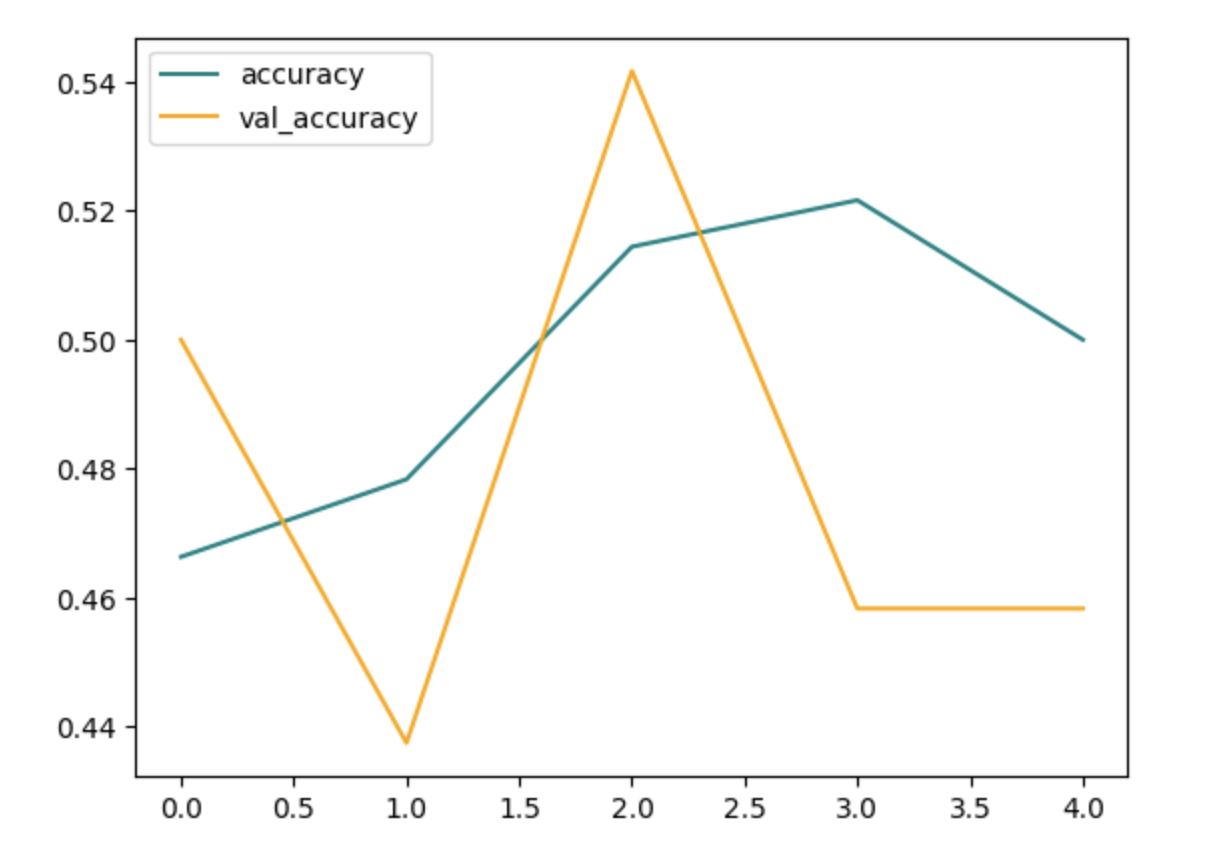
\includegraphics[keepaspectratio, scale=0.32]{ex1_acc.png}
    \caption{Composite}
  \end{minipage}
  \begin{minipage}[b]{0.45\linewidth}
    \centering
    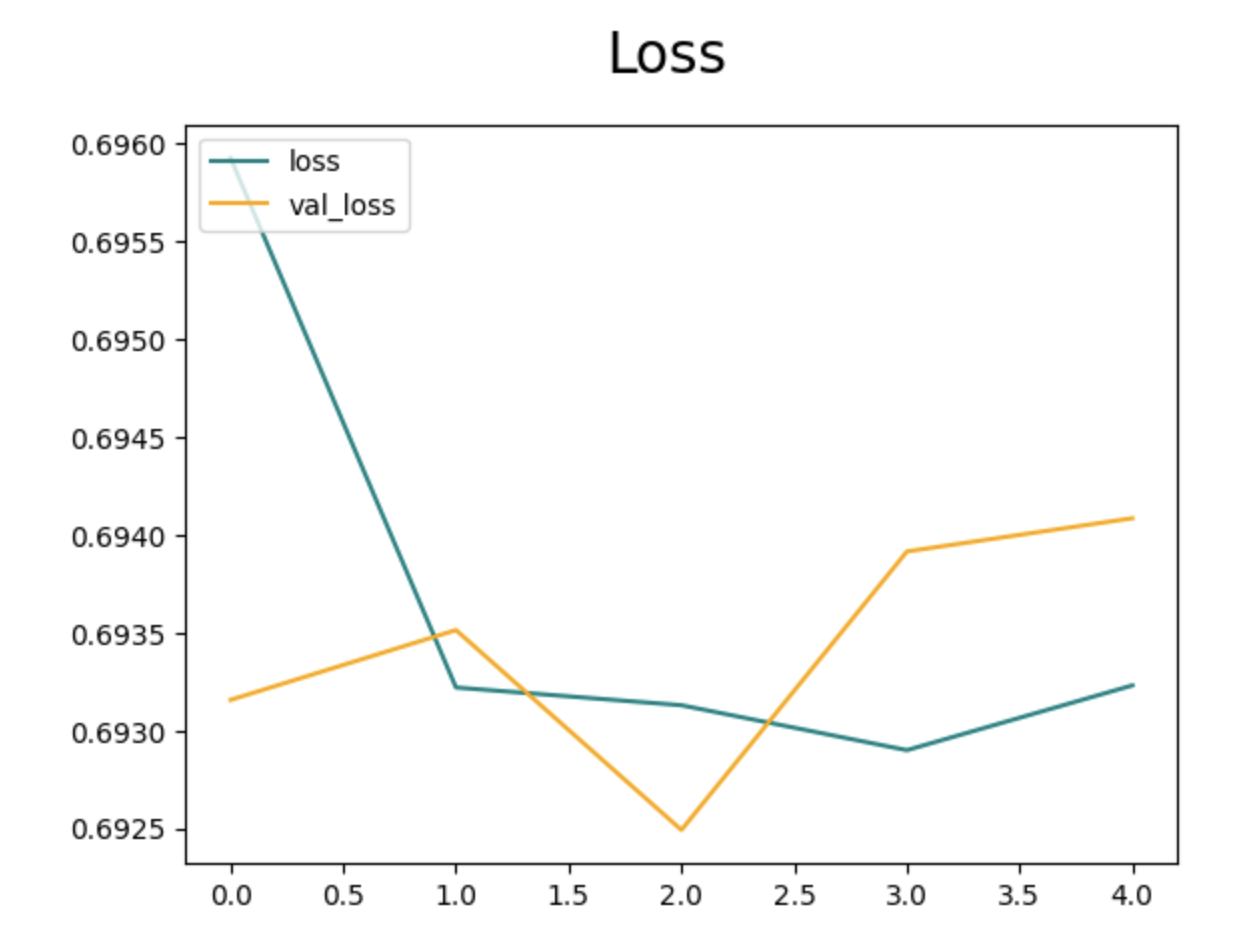
\includegraphics[keepaspectratio, scale=0.32]{ex1_loss.png}
    \caption{Gradation}
  \end{minipage}
\end{figure}

\subsection{実験2}
\begin{figure}[htbp]
  \begin{minipage}[b]{0.45\linewidth}
    \centering
    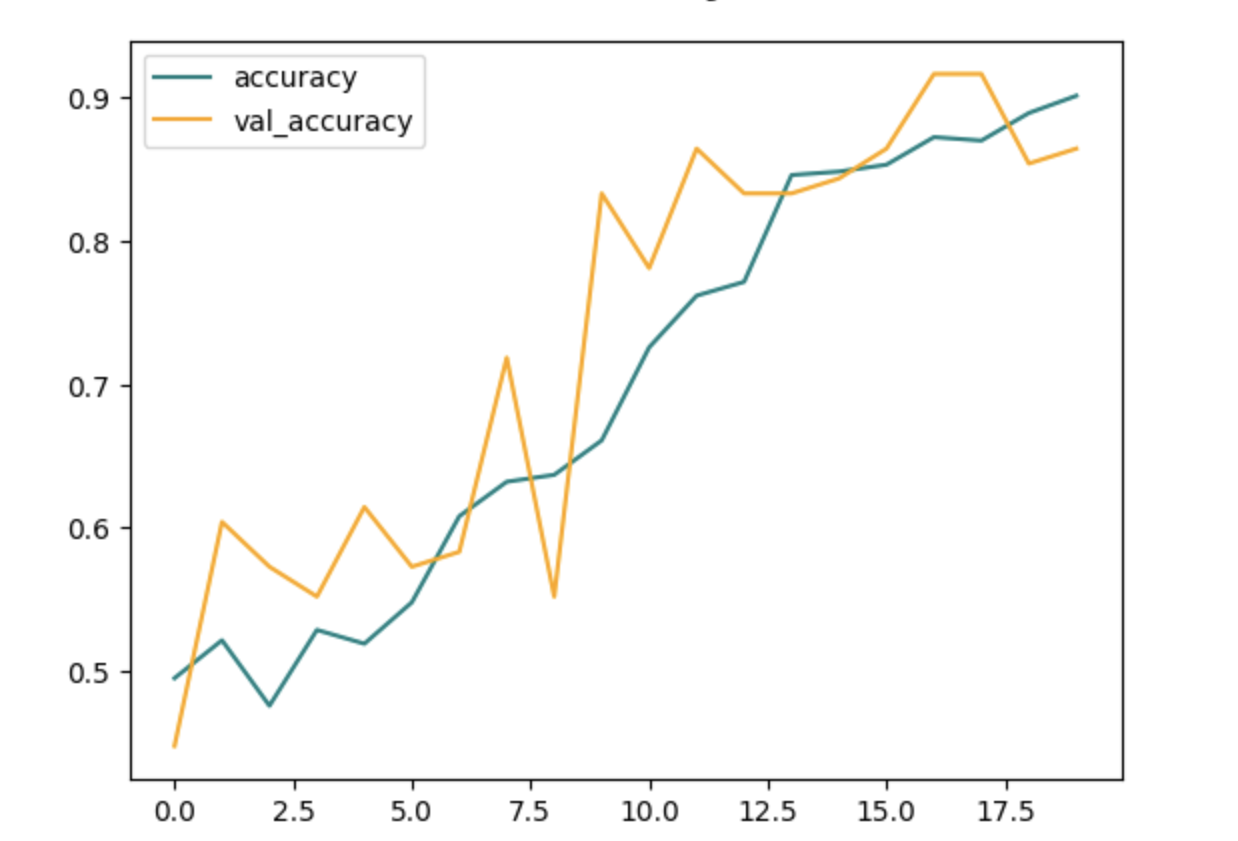
\includegraphics[keepaspectratio, scale=0.33]{ex2_acc.png}
    \caption{Composite}
  \end{minipage}
  \begin{minipage}[b]{0.45\linewidth}
    \centering
    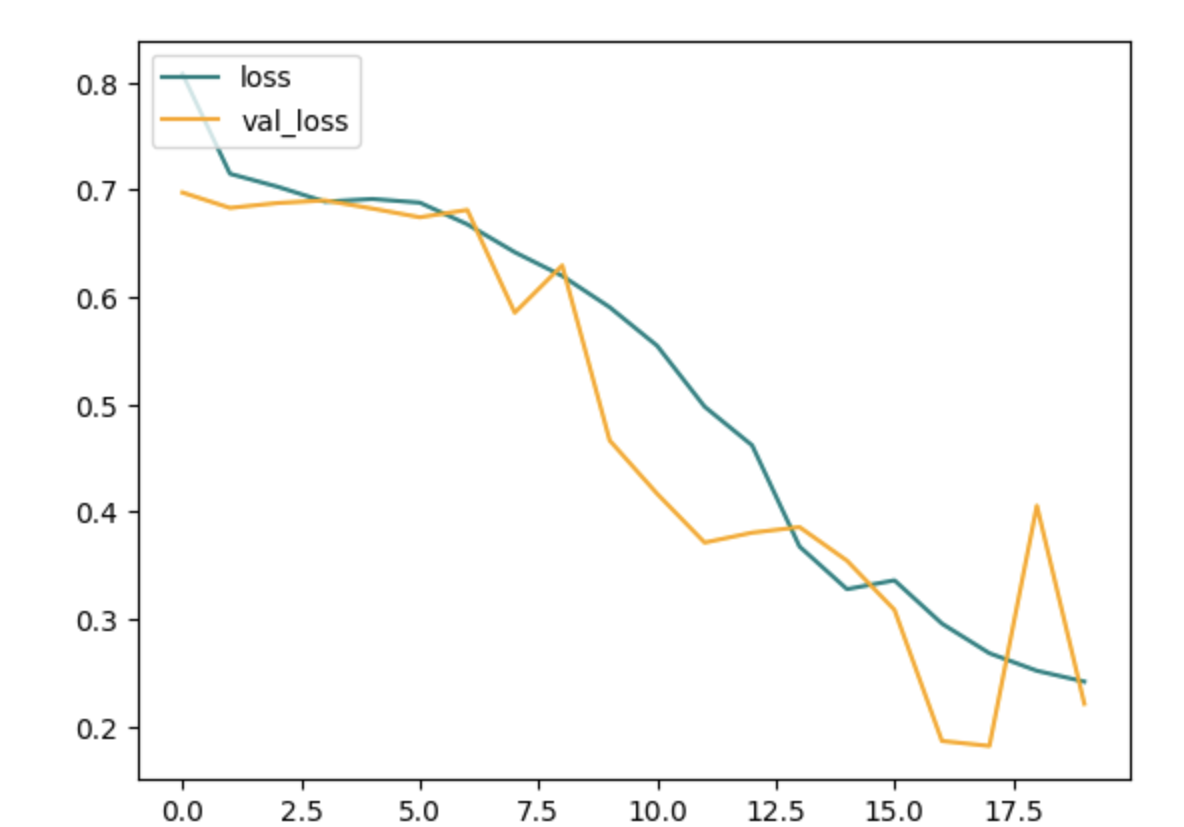
\includegraphics[keepaspectratio, scale=0.33]{ex2_loss.png}
    \caption{Gradation}
  \end{minipage}
\end{figure}

\subsection{実験3}
\begin{figure}[htbp]
  \begin{minipage}[b]{0.45\linewidth}
    \centering
    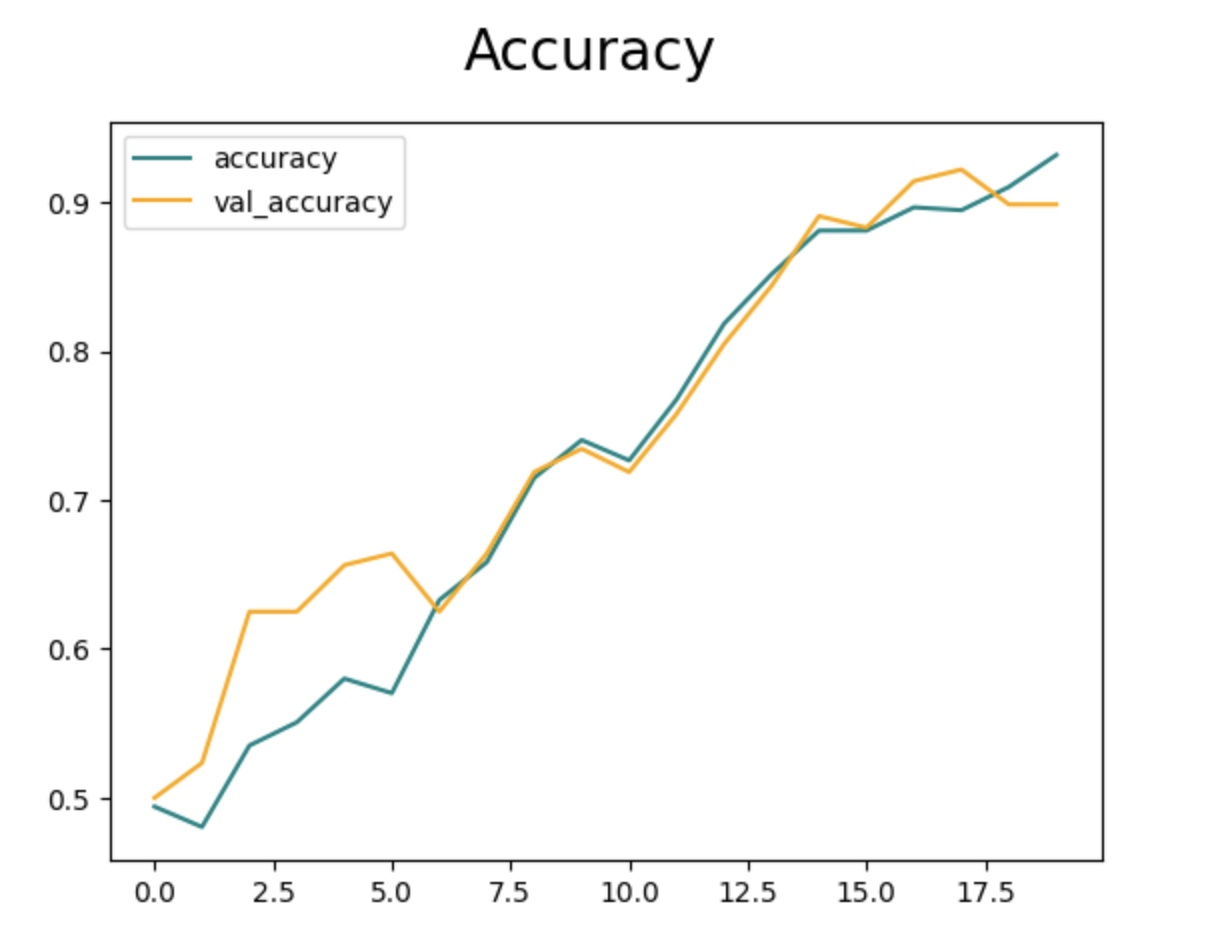
\includegraphics[keepaspectratio, scale=0.161]{ex3_acc.jpg}
    \caption{Composite}
  \end{minipage}
  \begin{minipage}[b]{0.45\linewidth}
    \centering
    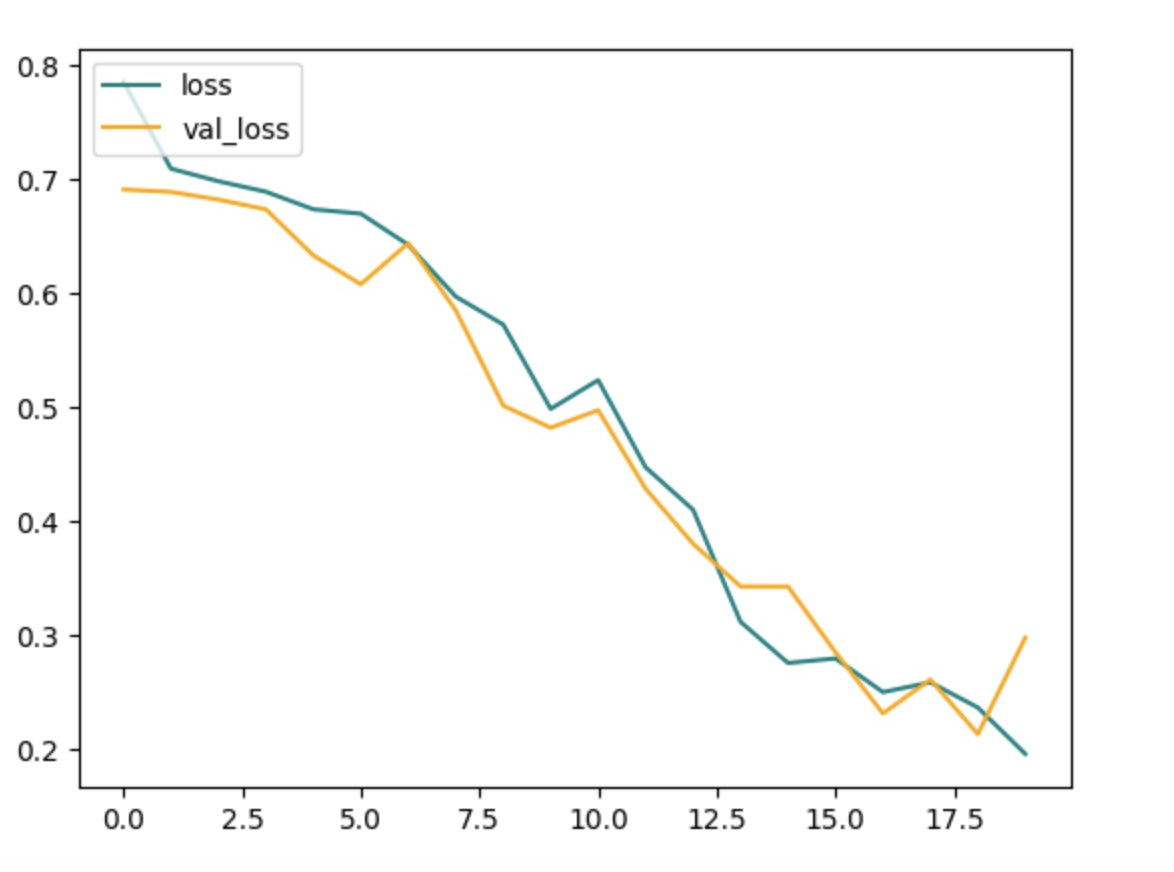
\includegraphics[keepaspectratio, scale=0.161]{ex3_loss.jpg}
    \caption{Gradation}
  \end{minipage}
\end{figure}

\subsection{実験4}
\begin{figure}[htbp]
  \begin{minipage}[b]{0.45\linewidth}
    \centering
    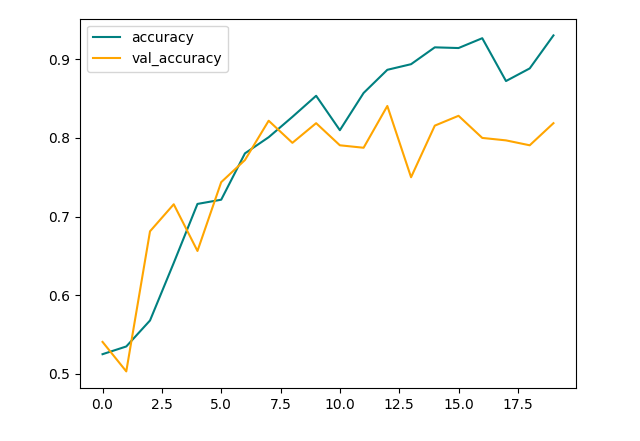
\includegraphics[keepaspectratio, scale=0.435]{ex4_acc.png}
    \caption{Composite}
  \end{minipage}
  \begin{minipage}[b]{0.45\linewidth}
    \centering
    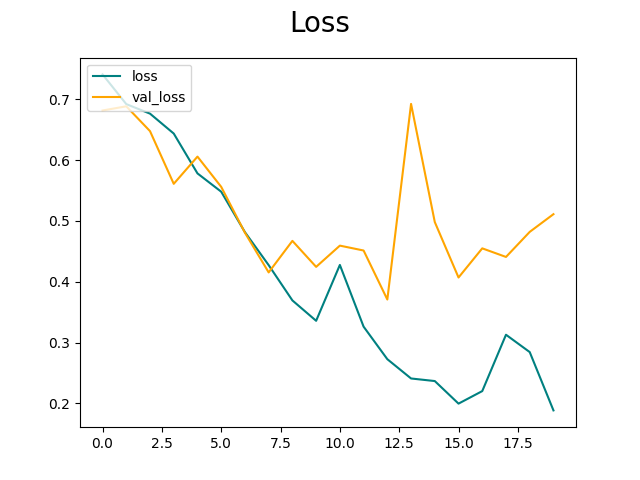
\includegraphics[keepaspectratio, scale=0.435]{ex4_loss.png}
    \caption{Gradation}
  \end{minipage}
\end{figure}

\section{考察}


\section{意図していた実験計画との違い}
行った実験の流れをガントチャートを用いて、表すと以下の通りになった。\par
\begin{figure}[htbp]
\begin{center}
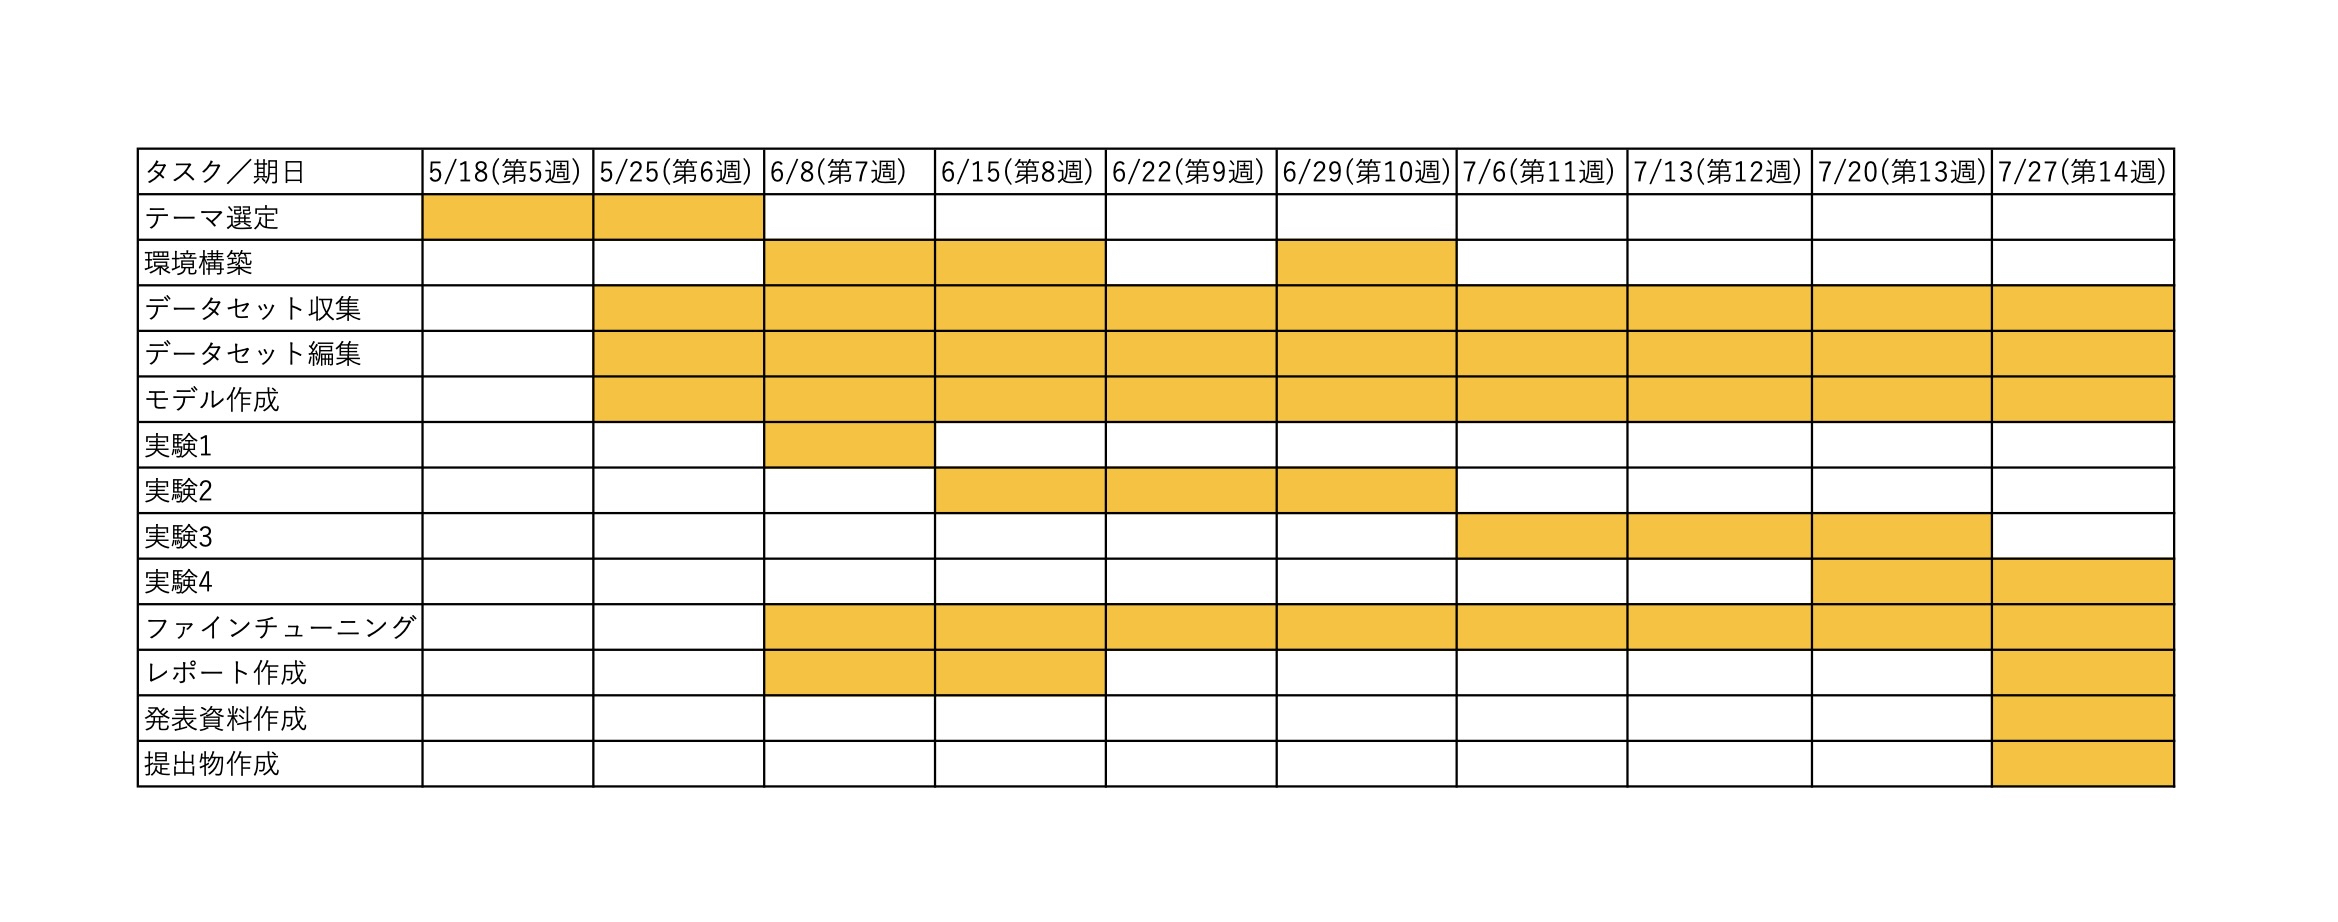
\includegraphics[width=150mm]{G2_Ganttchart.jpeg}
\caption{行った実験の流れ}
\end{center}
\end{figure}
想定していた以上に環境構築で躓いてしまい、本来1週で構築する予定だったが3週ほどかかってしまった。データセットに関しては、開発期間全体を通して収集・編集をおこない、正答率向上を目指した。

\section{まとめ}


\begin{thebibliography}{n}
  \bibitem{kanazawa}レポート作成の手引き レポートの基本的形式に関するガイド, \url{https://www.kanazawa-u.ac.jp/wp-content/uploads/2015/01/tebiki2.pdf}, 2020/07/02.
	\bibitem{theme1}画像認識でよく聞く「CNN」とは?仕組みや特徴を1から解説, \url{https://aismiley.co.jp/ai_news/cnn/}, 2023/06/14.
	\bibitem{theme2}画像認識の分野では欠かせない「CNN(畳み込みネットワーク)とは」, \url{https://www.paloaltoinsight.com/2022/12/09/cnn/},2023/06/14.
\end{thebibliography}
\end{document}
